% !TEX root = /media/ueslei/Ueslei/INPE/PCI/Projetos/Guia_COAWST/main.tex
\chapterimage{header.jpg}
\chapter{Building the ROMS}\index{Building the ROMS}
\bigskip
\section{Installing Python libraries on the personal computer}
\bigskip

\noindent Before generating the ROMS files, it is necessary to install the libraries and modules. 
In this chapter, we address how to download them, as well as the commands in the terminal to install through \textit{apt-get}.
\bigskip

\noindent There are two ways to install the required libraries: manually, and through Anaconda. 
Anaconda is a free and open source platform for Python and R and has a package manager called Conda, which makes easy 
to install the libraries. In this guide, I will present both options. For convenience, I suggest installing using Conda 
(Section \textcolor{bleu_cite}{\ref{condasec}}), but beware of version conflicts, as the Conda repositories are constantly updated.
\bigskip

\begin{tcolorbox}[enhanced,
  grow to left by   = 0cm,
  grow to right by  = 0cm,
  enlarge top by    = 0cm,
  enlarge bottom by = 0cm,
  tcbox raise base,
  boxrule           = 1.0pt,
  left              = 18mm,
  colframe          = red!50!black,coltext=red!25!black,colback=red!10!white,
  overlay           = {\begin{tcbclipinterior}\fill[red!75!blue!50!white] (frame.south west)
    rectangle node[text=white,font=\sffamily\bfseries\footnotesize,rotate=0] {WARNING} ([xshift=18mm]frame.north west);\end{tcbclipinterior}}]
ROMS files must be builded on your own computer and no longer on Kerana cluster, as previously done with WRF.
\end{tcolorbox}
\bigskip

\subsection{Installing manually}\index{Instalação manual}
\bigskip
\begin{tcolorbox}[enhanced,
    grow to left by   = 0cm,
    grow to right by  = 0cm,
    enlarge top by    = 0cm,
    enlarge bottom by = 0cm,
    tcbox raise base,
    boxrule           = 1.0pt,
    left              = 18mm,
    colframe          = red!50!black,coltext=red!25!black,colback=red!10!white,
    overlay           = {\begin{tcbclipinterior}\fill[red!75!blue!50!white] (frame.south west)
      rectangle node[text=white,font=\sffamily\bfseries\footnotesize,rotate=0] {WARNING} ([xshift=18mm]frame.north west);\end{tcbclipinterior}}]
Consider installing libraries with Anaconda will be faster than installing manually. See Section \textcolor{bleu_cite}{\ref{condasec}}.
  \end{tcolorbox}
\bigskip


\subsection{Installing with Conda}\label{condasec}
\bigskip
\noindent Anaconda is a distribution for Python and R that supports the various libraries and packages used in this guide, 
making installation easier. To download Anaconda go to
\textcolor{bleu_cite}{\href{https://www.continuum.io/downloads}{\textit{https://www.continuum.io/downloads}}}. 
To install, just enter the directory where the installation file is located, change the installation permissions of the file and 
follow the installer's instructions:
\bigskip

\begin{bashcode}
 sudo chmod 770 Anaconda2.sh
 ./Anaconda2.sh
\end{bashcode}
\bigskip

\noindent Next, enter the following commands on the terminal to install the libraries needed to build a project on ROMS using Python:
\bigskip

\begin{bashcode}
conda install -c conda-forge openmpi
conda install -c anaconda gcc
conda install -c mutirri szip
conda install -c anaconda zlib
conda install -c anaconda curl
conda install -c anaconda hdf5
conda install -c conda-forge netcdf-fortran
conda install -c scitools jasper
conda install -c anaconda libpng
conda install -c conda-forge udunits
conda install -c anaconda netcdf4
conda install -c anaconda cython
conda install -c anaconda numpy
conda install -c anaconda scipy
conda install -c anaconda mpi4py
conda install -c conda-forge esmf
conda install -c conda-forge lpsolve55 
conda install -c conda-forge cftime
\end{bashcode}
\bigskip

\section{Installing Pyroms}\index{Instalando o Pyroms}
\bigskip

\noindent With the libraries already installed, this section will show you how to install Pyroms. 
It is a collection of tools to create ROMS files. It was originally started by Rob Hetland as a project on GoogleCode and 
rewritten by Frederic Castruccio.
\bigskip

\noindent Pyroms can be easily installed using Pip, a command line tool that allows you to install software packages written in Python.
To install Pip for Python 2, use the following:
\bigskip

\begin{bashcode}
  sudo apt install python-pip
\end{bashcode}
\bigskip

\noindent For Python 3 users, use:
\bigskip
\begin{bashcode}
sudo apt install python3-pip
\end{bashcode}
\bigskip

\noindent Then, install the Pyrons by cloning the repository at Github:
\bigskip

\begin{bashcode}
git clone https://github.com/ESMG/pyroms.git
\end{bashcode}
\bigskip

\noindent Install it using Pip:
\bigskip

\begin{bashcode}
pip install -e pyroms/pyroms
pip install -e pyroms/pyroms_toolbox
pip install -e pyroms/bathy_smoother
\end{bashcode}
\bigskip

\noindent This will install both three Pyroms packages, but if you try to import any of then without Script installed, you will get a warning 
similar to that found in \textcolor{bleu_cite}{Figure \ref{scriperror}}:
\bigskip

\begin{figure}[H]
  \centering
  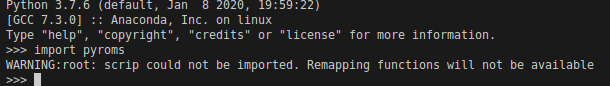
\includegraphics[width=0.85\textwidth]{scriperror.png}
  \caption{Scrip warning when Pyroms is imported without installing it.}
  \label{scriperror}
\end{figure}
\bigskip

\noindent As stated in the Pyroms repository, the scrip module is not available via Conda or any other package repository, but it can be built 
and installed from source as the following:
\bigskip

\begin{bashcode}
cd pyroms/pyroms/external/scrip/source/
\end{bashcode}
\bigskip

\noindent Then, print the active Conda environment path. This will be used to find the netCDF library.
\bigskip

\begin{bashcode}
conda info | grep "active env location"
\end{bashcode}
\bigskip

\noindent The output must be something like as the following:
\bigskip

\begin{bashcode}
active env location : /home/USER/anaconda3
\end{bashcode}
\bigskip

\noindent Export the PREFIX variable with the location found in the previous step.
\bigskip

\begin{bashcode}
export PREFIX=/home/USER/anaconda3
\end{bashcode}
\bigskip

\noindent Install the module with the make command.
\bigskip

\begin{bashcode}
sudo make DEVELOP=1 PREFIX=$PREFIX install
\end{bashcode}
\bigskip

\noindent Move the Scrip files to the Pyroms folder, like the following:
\bigskip

\begin{bashcode}[fontsize=\scriptsize]
  mv -vf scrip*.so ../../../pyroms
  ‘scrip.cpython-37m-x86_64-linux-gnu.so’ -> ‘../../../pyroms/scrip.cpython-37m-x86_64-linux-gnu.so’
\end{bashcode}
\bigskip

\section{The model2roms toolbox}\index{O model2roms}\label{model2romssec}
\bigskip

\noindent In this section, you will be introduced to install model2roms, the toolbox used to generate ROMS forcing files and its grid. 
It was created and is being updated by Trond Kristiansen (\textcolor{bleu_cite}{\cite{Trond2019}}) and we adapted to the needs of 
LOA-INPE. 
\bigskip

\noindent To download \textit{model2roms}, enter \textit{home} on your computer and download using Github:
\bigskip

\begin{bashcode}
cd $HOME
git clone https://github.com/usutil/model2roms
\end{bashcode}
\bigskip

\noindent Change the folder name from \textit{model2roms-master} to \textit{model2roms}:
\bigskip

\begin{bashcode}
mv model2roms-master model2roms
\end{bashcode}
\bigskip

\subsection{Introduction to the ROMS grid}\index{Gerar a grade do ROMS}
\bigskip

\noindent To generate the ROMS grid, we will use the code \textit{make\_roms\_grid.py}, located in the \textit{model2roms/grid} 
directory. The code supports the SRTM30\_plus data (\cite{Becker2009}), however, for practical purposes, we will exemplify 
only the data from ETOPO1 (\cite{Amante2009}), which will be discussed in the next subsection.
\bigskip

\noindent Install basemap to use the code, if you have not previously installed
\bigskip

\begin{bashcode}
conda install -c anaconda basemap
\end{bashcode}
\bigskip

\subsection{ETOPO1 1 Arc-Minute Global Relief Model}\index{O ETOPO1 1 Arc-Minute Global Relief Model}
\bigskip

\noindent The ETOPO1 (\cite{Amante2009}; Figure \textcolor{bleu_cite}{\ref{etopo1}}) 
is produced by the National Geophysical Data Center and provides two layers of relief information.
The layers include bathymetry over the oceans and some of the main lakes on Earth.
 Terrestrial topography and ocean bathymetry are based on SRTM30 topography and through various bathymetric cruises
\bigskip

\noindent Visit the site \textcolor{bleu_cite}{\href{https://www.ngdc.noaa.gov/mgg/global/global.html}{\textit{https://www.ngdc.noaa.gov/mgg/global/global.html}}} 
and subset your area of interes on the ETOPO1 website map and download the data in NetCDF format.

\bigskip  
   
\begin{figure}[H]
    \centering
    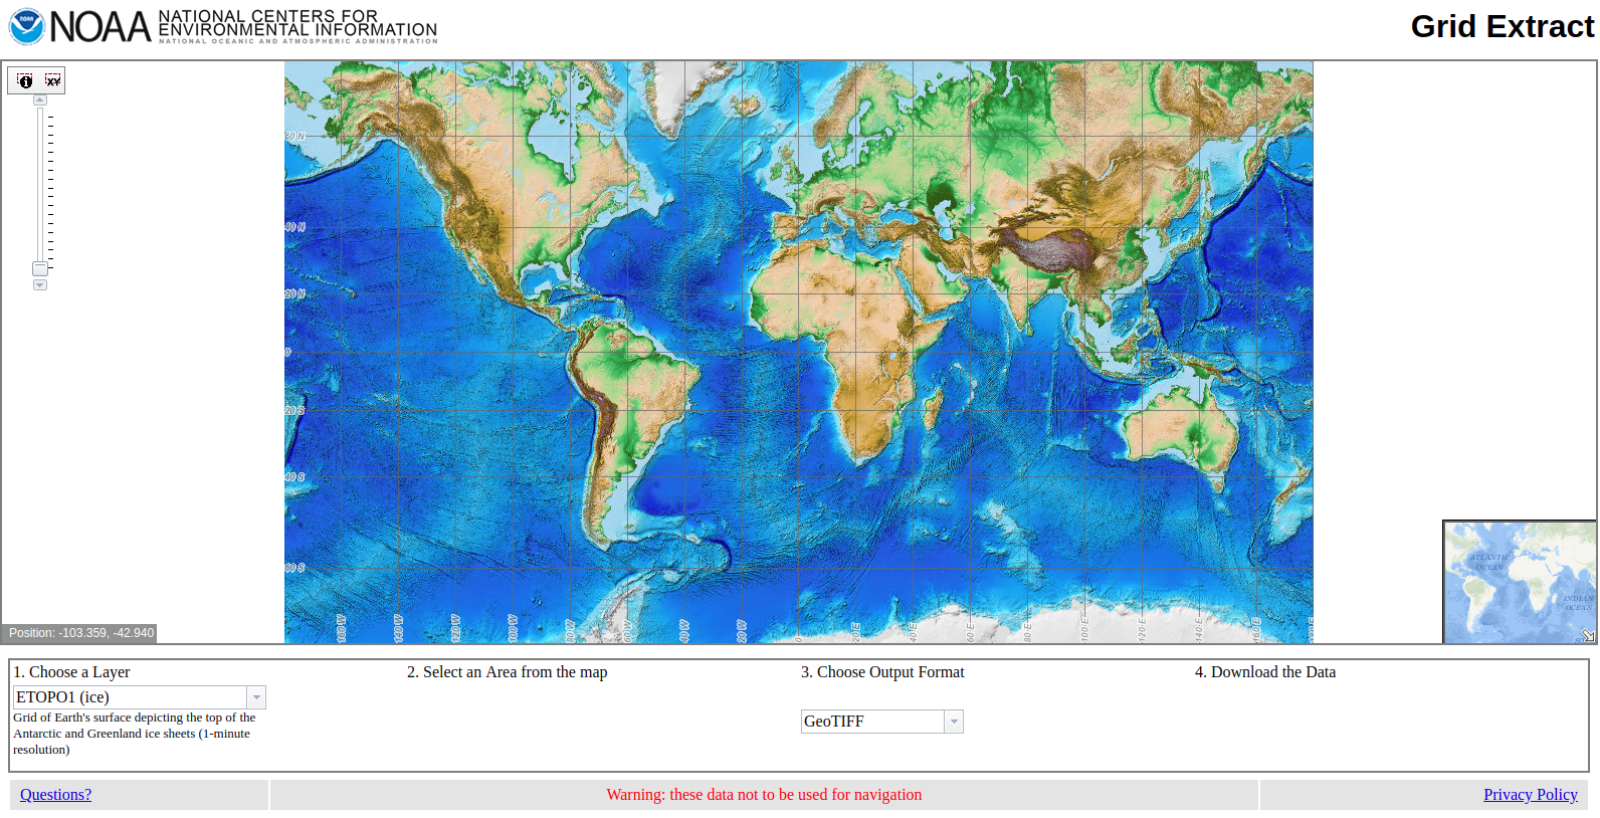
\includegraphics[width=0.85\textwidth]{etopo1.png}
    \caption{ETOPO1 webpage.}
    \label{etopo1}
\end{figure}
\bigskip


\bigskip

\begin{tcolorbox}[enhanced,
    grow to left by   = 0cm,
    grow to right by  = 0cm,
    enlarge top by    = 0cm,
    enlarge bottom by = 0cm,
    tcbox raise base,
    boxrule           = 1.0pt,
    left              = 18mm,
    colframe          = red!50!black,coltext=red!25!black,colback=red!10!white,
    overlay           = {\begin{tcbclipinterior}\fill[red!75!blue!50!white] (frame.south west)
      rectangle node[text=white,font=\sffamily\bfseries\footnotesize,rotate=0] {WARNING} ([xshift=18mm]frame.north west);\end{tcbclipinterior}}]
The script \textit{make\_roms\_grid.py} does not allow the selection of the latitude and longitude limits of the grid, therefore, be as accurate as possible when subseting of your area.

\end{tcolorbox}
\bigskip

\subsubsection{Creating the ROMS grid}\index{Gerando a grade do ROMS}

\noindent Enter the \textit{model2roms} directory and look for the \textit{grid} subfolder. Open the code \textit{make\_roms\_grid.py}.
\bigskip

\begin{bashcode}
cd $HOME/model2roms/grid
gedit make_roms_grid.py
\end{bashcode}
\bigskip

\noindent As Figure \textcolor{bleu_cite}{\ref{fazgrade}} shown, the variables that will be modified are:
\bigskip

\begin{itemize}
\item \textbf{grd\_name}: Grid name;
\item \textbf{grd\_final}: The NetCDF file name of the grid;
\item \textbf{etopo1\_dir}: The directory where the ETOPO1 NetCDF file is located;
\item\textbf{srtm\_dir}: The directory where the SRTM\_30\_PLUS NetCDF file is located; 
\item \textbf{hmin}: Value of \textit{h} parameter;
\item \textbf{theta\_b}: Control parameter for coordinates close to the ocean floor;
\item \textbf{theta\_s}: Control parameter for coordinates close to the surface;
\item \textbf{Tcline}: Critical depth, in meters, controlling the elongation of the coordinates following the terrain. It can be interpreted as the width of the surface where vertical resolution is best;
\item \textbf{N}: Number of Sigma layers;
\item \textbf{rmax}: Topography smoothing factor;
\item \textbf{intrp\_method}: Grid interpolation method: Linear (\textit{linear}) or Near Neighbor (\textit{nn});
\item \textbf{grid\_resolution}: Grid resolution;
\item\textbf{max\_depth}: Maximum grid depth.
\end{itemize}
\bigskip

\begin{tcolorbox}[enhanced,
    grow to left by   = 0cm,
    grow to right by  = 0cm,
    enlarge top by    = 0cm,
    enlarge bottom by = 0cm,
    tcbox raise base,
    boxrule           = 1.0pt,
    left              = 18mm,
    colframe          = red!50!black,coltext=red!25!black,colback=red!10!white,
    overlay           = {\begin{tcbclipinterior}\fill[red!75!blue!50!white] (frame.south west)
      rectangle node[text=white,font=\sffamily\bfseries\footnotesize,rotate=0] {WARNING} ([xshift=18mm]frame.north west);\end{tcbclipinterior}}]
      In \textit{grid\_resolution}, it is necessary to place the numerator to do the ETOPO1 calculation. For example: as ETOPO1 has 1/60° of spatial resolution, if the chosen spatial resolution is 1/12°, the value of \textit{grid\_resolution} will be 5, because 5/60° is the same as 1/12° .\end{tcolorbox}
\bigskip

\begin{tcolorbox}[enhanced,
    grow to left by   = 0cm,
    grow to right by  = 0cm,
    enlarge top by    = 0cm,
    enlarge bottom by = 0cm,
    tcbox raise base,
    boxrule           = 1.0pt,
    left              = 18mm,
    colframe          = red!50!black,coltext=red!25!black,colback=red!10!white,
    overlay           = {\begin{tcbclipinterior}\fill[red!75!blue!50!white] (frame.south west)
      rectangle node[text=white,font=\sffamily\bfseries\footnotesize,rotate=0] {WARNING} ([xshift=18mm]frame.north west);\end{tcbclipinterior}}]
As we do not use the data from SRTM\_30\_PLUS, the variable \textit{srtm\_dir} does not need to be modified.
\end{tcolorbox}
\bigskip

\begin{figure}[H]
    \centering
    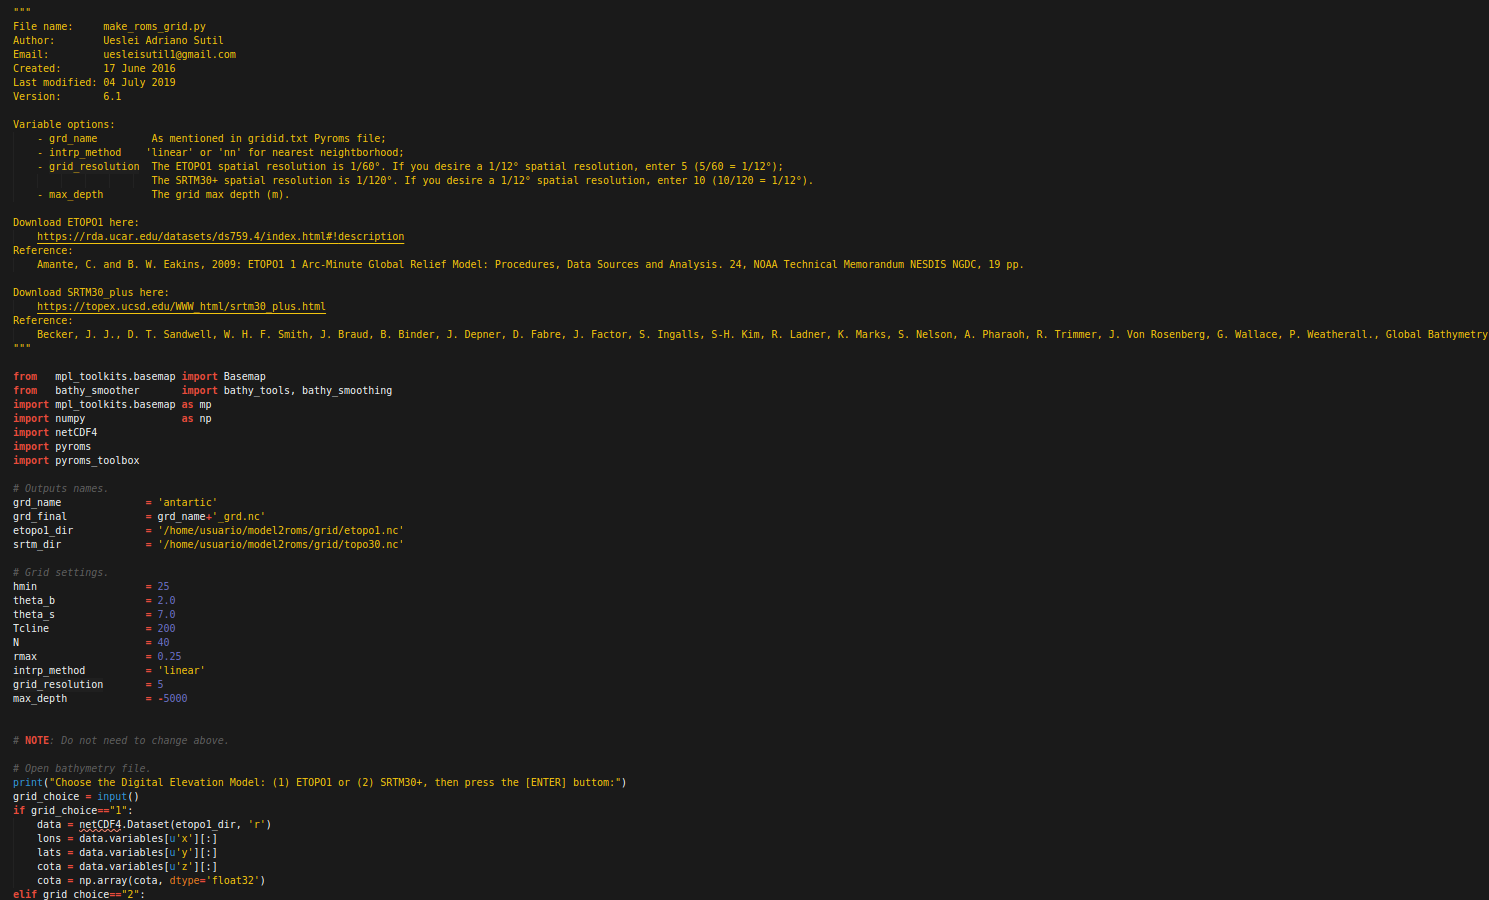
\includegraphics[width=1\textwidth]{makegrid.png}
    \caption{Screenshot of the \textit{make\_grid.py} file, which is located in the \textit{model2roms/grid} folder.}
    \label{fazgrade}
\end{figure}
\bigskip

\noindent After making the changes, just run the code. Type it:
\bigskip

\begin{bashcode}
ipython make_roms_grid.py --pylab
\end{bashcode}
\bigskip

\subsection{Introduction to ROMS forcing files}\index{Introdução sobre as condições do ROMS}
\bigskip

\noindent We will use \textit{model2roms} to generate the ROMS conditions. The toolbox supports data from GLORYS12V1 (\cite{Fernandez2018}) 
and SODA3 (\cite{Carton2018}), however, we will only use GLORYS12V1 as an example.

\subsection{Global Ocean Physics Reanalysis (GLORYS)}\index{O Global Ocean Physics Reanalysis (GLORYS)}
\bigskip

\noindent GLORYS is a global reanalysis of the ocean with a spatial resolution of 1/12° with daily or monthly temporal resolution and 
50 vertical levels. It is based on the current CMEMS global weather forecasting system and is forced by ECMWF's ERA-Interim from the NEMO model.
A Kalman filter with reduced order is used to assimilate the sea altimetry, sea surface temperature, sea ice concentration data obtained 
from remote sensing and the \textit{in situ} data of vertical temperature and salinity profiles .
In addition, a 3D-VAR scheme provides a correction for temperature and salinity deviations.
\bigskip

\noindent GLORYS can be downloaded from the website: 
\textcolor{bleu_cite}{\href{http://marine.copernicus.eu/services-portfolio/access-to-products/?option=com\_csw\&view=details\&product\_id=GLOBAL\_REANALYSIS\_PHY\_001\_030}{\textit{http://marine.copernicus.eu/services-portfolio/access-to-products/?option=com\_csw\&view=details\&product\_id=GLOBAL\_REANALYSIS\_PHY\_001\_030}}}.
\bigskip

\noindent When you try to download, the site will warn you that you will need to create a Copernicus account.
Register and choose the GLORYS daily data set, as shown in Figure \textcolor{bleu_cite}{\ref{glorys1}}.
\bigskip

\begin{figure}[H]
    \centering
    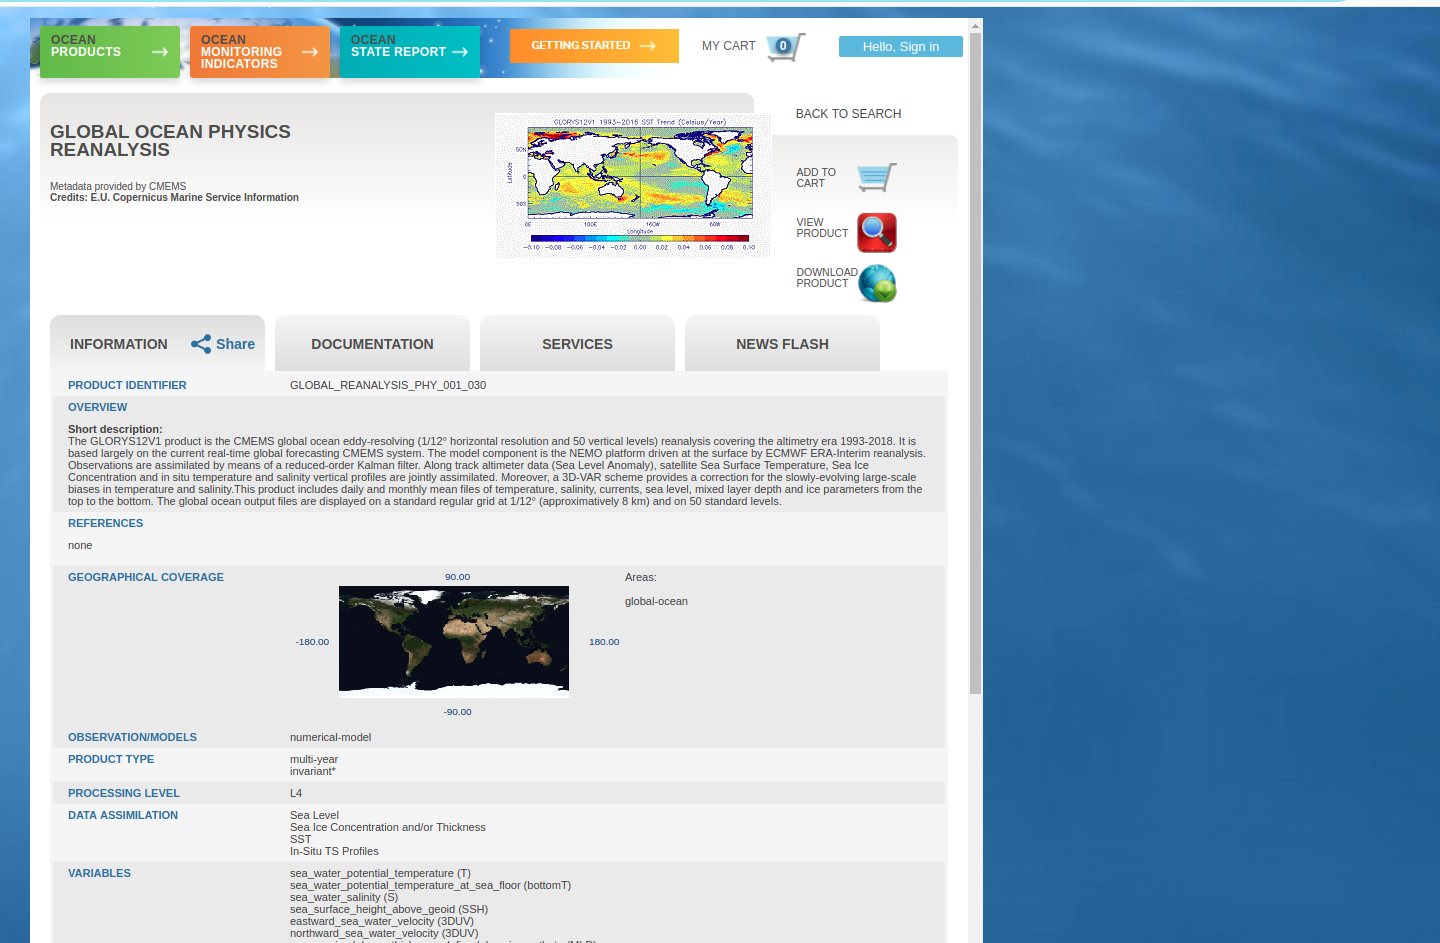
\includegraphics[width=0.7\textwidth]{glorys1.png}
    \caption{Screenshot from GLORYS webpage.}
    \label{glorys1}
\end{figure}
\bigskip

\noindent Click on \textit{Dowload product} and, on the next page (Figure \textcolor{bleu_cite}{\ref{glorys2}}), select the area according to 
the latitude and longitude limits of the chosen grid. Also choose the period of data to be downloaded and if you want to use the sea 
ice model in ROMS, select all variables, with the exception of:
\bigskip

\begin{itemize}
    \item \textit{ bottomT - Sea floor potential temperature};
    \item \textit{mlotst - Density ocean mixed layer thickness}.
\end{itemize}
\bigskip

\noindent If you choose to not use the sea ice model, do not select the variables:
\bigskip

\begin{itemize}
    \item \textit{siconc - Ice concentration};
    \item \textit{sithick - Sea ice thickness};
    \item \textit{usi - Sea ice eastward velocity};
    \item \textit{vsi - Sea ice northward velocity}.
\end{itemize}
\bigskip

\begin{figure}[H]
    \centering
    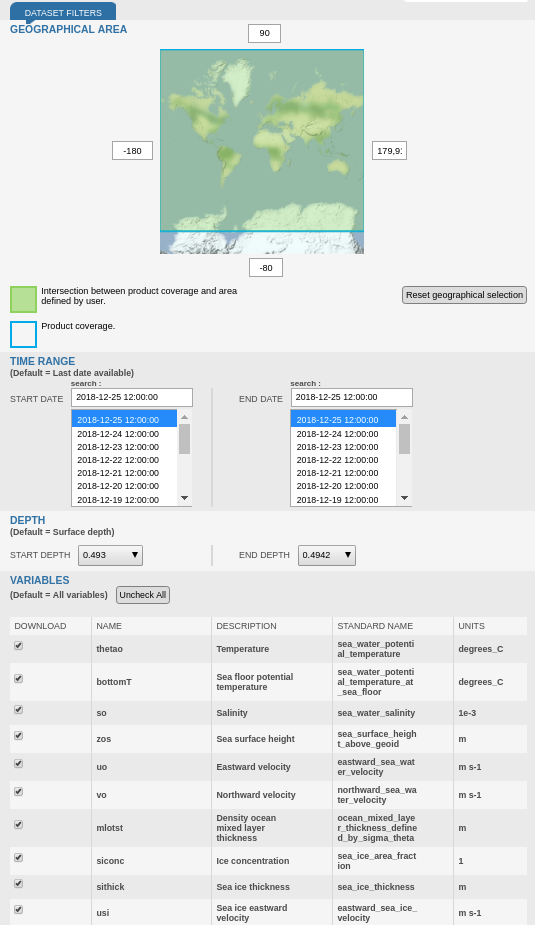
\includegraphics[width=0.5\textwidth]{glorys2.png}
    \caption{Another screenshot from the GLORYS webpage.}
    \label{glorys2}
\end{figure}
\bigskip

\noindent The Copernicus server allow files for download with a maximum of 1024 mb. 
If the selected period has a larger file size, as for example in Figure \textcolor{bleu_cite}{\ref{glorys3}}, it will be necessary to 
return to the previous step and partition the files into smaller pieces or download the complete file by clicking on \textit{FTP ACCESS}
(Figure \textcolor{bleu_cite}{\ref{glorys3}}).
\bigskip

\begin{figure}[H]
    \centering
    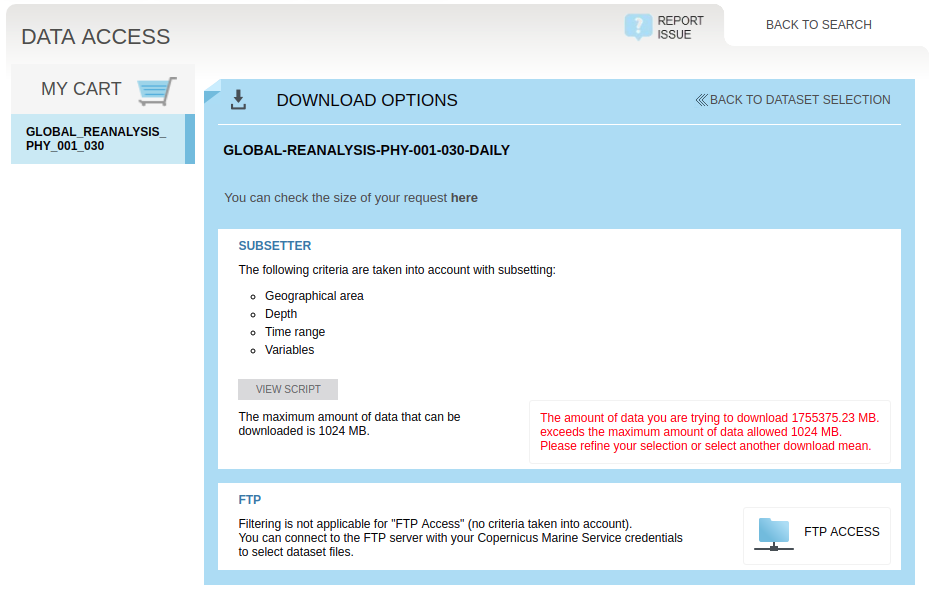
\includegraphics[width=0.6\textwidth]{glorys3.png}
    \caption{Error message when trying to download a text larger than 1024 mb.}
    \label{glorys3}
\end{figure}
\bigskip

\noindent If you choose to partition the files or download the files by \textit{FTP}, you will need to create a new file with 
all the concatenated chosen dates. In this case, it is necessary to use \textit{Climate Data Operators} (CDO).
\bigskip

\noindent There are two ways to install CDO: by \textit{Conda} or by \textit{apt-get}.
\bigskip

\noindent If you choose to use \textit{Conda}, type:
\bigskip

\begin{bashcode}
conda install -c conda-forge cdo
\end{bashcode}
\bigskip

\noindent If you choose to use \textit{apt-get}, type:
\bigskip

\begin{bashcode}
sudo apt-get install cdo
\end{bashcode}
\bigskip

\noindent After installation, enter the directory where all GLORYS files are located and type:
\bigskip

\begin{bashcode}
cdo cat glorys* glorys.nc
\end{bashcode}
\bigskip

\noindent Where: 
\bigskip

\begin{itemize}
    \item  \textit{cdo} means the program command;
    \item \textit{cat} means the concatenation command of all files;
    \item \textit{glorys*} means that all files called \textit{glorys} will be concatenated within the folder;
    \item \textit{glorys.nc} means the final file name created by concatenating with \textit{CDO}.
\end{itemize}
\bigskip

\begin{tcolorbox}[enhanced,
    grow to left by   = 0cm,
    grow to right by  = 0cm,
    enlarge top by    = 0cm,
    enlarge bottom by = 0cm,
    tcbox raise base,
    boxrule           = 1.0pt,
    left              = 18mm,
    colframe          = red!50!black,coltext=red!25!black,colback=red!10!white,
    overlay           = {\begin{tcbclipinterior}\fill[red!75!blue!50!white] (frame.south west)
      rectangle node[text=white,font=\sffamily\bfseries\footnotesize,rotate=0] {WARNING} ([xshift=18mm]frame.north west);\end{tcbclipinterior}}]
  Para facilitar os próximos passos, coloque o arquivo do GLORYS dentro do diretório \textit{\$HOME/model2roms/input}
\end{tcolorbox}

\subsection{Creating ROMS forcing files}\index{Gerando as condições do ROMS}
\bigskip

\noindent When opening the \textit{model2roms} folder, it is possible to observe several script files. 
We will start with the file \textit{compile.py}, which will compile several files in Fortran90. 
\bigskip

\noindent Compile the files with the command:
\bigskip

\begin{bashcode}
ipython compile.py --pylab
\end{bashcode}
\bigskip

\noindent If your \textit{GLORYS} file name is different from \textit{glorys.nc}, open the code \textit{forcingFilenames.py} 
(Figure \textcolor{bleu_cite}{\ref{forcingfilename}}) and in row 15, change \textit{'glorys.nc'} to the name of the created file.
\bigskip

\begin{bashcode}
cd $HOME/model2roms
gedit forcingFilenames.py
\end{bashcode}
\bigskip

\begin{figure}[H]
    \centering
    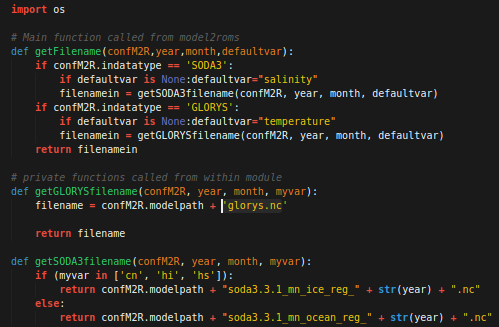
\includegraphics[width=0.6\textwidth]{forcingfilename.png}
    \caption{Screenshot of the \textit{forcingFilename.py} file.}
    \label{forcingfilename}
\end{figure}
\bigskip

\noindent Open the file \textit{configM2R.py} and, in row 16 (Figure \textcolor{bleu_cite}{\ref{abrev}}), change the abbreviation \textit{SuaAbreviaçãoAqui} 
of the \textit{defineabbreviation} to the name of your choice.
\bigskip

\begin{figure}[H]
    \centering
    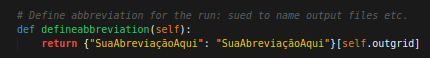
\includegraphics[width=0.6\textwidth]{abrevi.png}
    \caption{Screenshot of the \textit{defineabbreviation} in the code \textit{configM2R.py}.}
    \label{abrev}
\end{figure}
\bigskip

\noindent In row 63 (Figure \textcolor{bleu_cite}{\ref{gradediretoriom2r}}), change the grid directory \textit{Minha\_Grade.nc} to your 
grid directory and the abbreviation \textit{SuaAbreviaçãoAqui} by the name chosen in the previous step.
\bigskip

\begin{figure}[H]
    \centering
    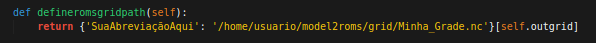
\includegraphics[width=0.6\textwidth]{m2rgriddir.png}
    \caption{Screenshot of the \textit{configM2R.py} code.
    }
    \label{gradediretoriom2r}
\end{figure}
\bigskip

\noindent On row 67 (Figure \textcolor{bleu_cite}{\ref{glorysdirm2r}}), change the \textit{GLORYS} file directory to your chosen path.
\bigskip

\begin{figure}[H]
    \centering
    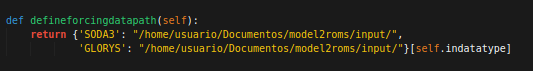
\includegraphics[width=0.6\textwidth]{glorysdirm2r.png}
    \caption{Screenshot of the \textit{configM2R.py} code.}
    \label{glorysdirm2r}
\end{figure}
\bigskip

\noindent From row 76 (Figure \textcolor{bleu_cite}{\ref{m2roptions}}), modify according to your project: 
\bigskip

\begin{itemize}
    \item \textbf{self.compileall}: Set as \textit{True} if you want the Fortran files to be recompiled each time \textit{model2roms} is executed;
    \item \textbf{self.createoceanforcing}: Set as \textit{True} to create the hydrodynamic variables;
    \item \textbf{self.createatmosforcing}: Set as \textit{True} to create atmospheric forces. \textbf{Currently this function is in the testing phase and is not entirely available for use};
    \item \textbf{self.writeice}: Set as \textit{True} to create the sea ice variables;
    \item \textbf{self.set2DvarsToZero}: Creates the ice and sea level files with zero values. Since GLORYS has these values, it is recommended to leave it as \textit{False};
    \item \textbf{self.useesmf}: Set as \textit{True} to use \textit{ESMF} to interpolate the GLORYS data to the ROMS grid;
    \item \textbf{self.usefilter}: Set as \textit{True} to apply a filter to smooth out 2D fields.
    \item \textbf{self.myformat}: The extension for writing ROMS input files. It is, by default, \textit{NETCDF};
    \item \textbf{self.timefrequencyofinputdata}: The time frequency of the input data. If using GLORYS, write \textit{'day'};
    \item \textbf{self.indatatype}: The name of the data used to generate the forcing files. \textit{'GLORYS} or \textit{SODA3};
    \item \textbf{self.authorname}: The name of the user using \textit{model2roms};
    \item \textbf{self.authoremail}: The email of the user using \textit{model2roms};
    \item \textbf{self.ingridtype}: It will interpolate the GLORYS grid, which is in \textit{'ZLEVEL'} coordinate;
    \item \textbf{self.grdtype}: The GLORYS grid type, which is \textit{'regular'};
    \item \textbf{self.lonname}: The name of the GLORYS longitude variable, which is \textit{'longitude'};
    \item \textbf{self.latname}: The name of the GLORYS latitude variable, which is \textit{'latitude'};
    \item \textbf{self.depthname}: The name of the GLORYS depth variable, which is \textit{'depth'};
    \item \textbf{self.lonname\_u}: The name of the GLORYS U-longitude variable, which is \textit{'longitude'};
    \item \textbf{self.latname\_u}: The name of the GLORYS U-latitude variable, which is \textit{'latitude'};
    \item \textbf{self.lonname\_v}: The name of the GLORYS V-longitude variable, which is \textit{'longitude'};
    \item \textbf{self.latname\_v}: The name of the GLORYS U-latitude variable, which is \textit{'latitude'};
    \item \textbf{self.timename}: The name of the GLORYS time variable, which is \textit{'time'};
    \item \textbf{self.realm}: The realm in which \textit{model2roms} is being executed, in this case, \textit{'ocean'};
    \item \textbf{self.fillvaluein}: The \textit{fillvalue} value of the NetCDF file. By convention, \textit{-1.e20};
    \item \textbf{self.outgrid}: The name of the abbreviation used in the definition \textit{defineabbreviation};
    \item \textbf{self.outgridtype}: If \textit{"ROMS"}, it will create the output in the standard ROMS format;
    \item \textbf{self.nlevels}: The number of vertical levels in the grid. It must be the same as the one chosen in the code \textit{make\_roms\_grid.py};
    \item \textbf{self.vstretching}: It must be the same as the one chosen in the code \textit{make\_roms\_grid.py};
    \item \textbf{self.vtransform}: It must be the same as the one chosen in the code \textit{make\_roms\_grid.py};
    \item \textbf{self.theta\_s}: It must be the same as the one chosen in the code \textit{make\_roms\_grid.py};
    \item \textbf{self.theta\_b}: It must be the same as the one chosen in the code \textit{make\_roms\_grid.py};
    \item \textbf{self.tcline}: It must be the same as the one chosen in the code \textit{make\_roms\_grid.py};   
    \item \textbf{self.hc}: It must be the same as the one chosen in the code \textit{make\_roms\_grid.py};
    \item \textbf{self.start\_year}: The initial year of GLORYS data;
    \item \textbf{self.end\_year}: The final year of GLORYS data;
    \item \textbf{self.start\_month}: The initial month of GLORYS data;
    \item \textbf{self.end\_month}: The final month of GLORYS data;
    \item \textbf{self.start\_day}: The initial day of GLORYS data;
    \item \textbf{self.end\_day}: The final day of GLORYS data;
\end{itemize}
\bigskip

\begin{figure}[H]
    \centering
    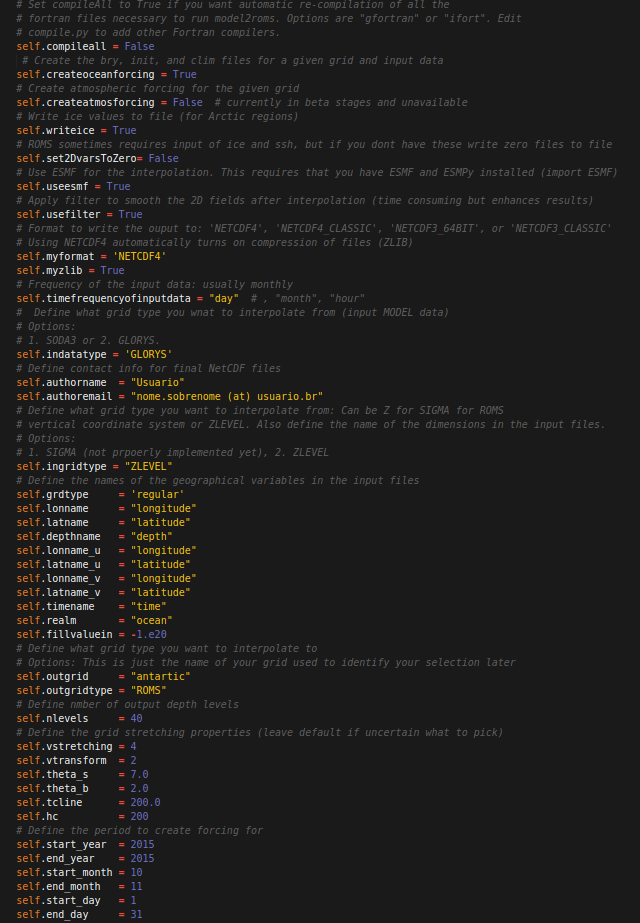
\includegraphics[width=0.5\textwidth]{m2roptions.png}
    \caption{Screenshot of the \textit{configM2R.py} code.}
    \label{m2roptions}
\end{figure}
\bigskip

\noindent Run \textit{model2roms} with the command:
\bigskip

\begin{bashcode}
ipython runM2R.py
\end{bashcode}
\bigskip

\noindent At the end, the initial, boundary and climatological files will be created, which should be added to your project folder, in the Kerana cluster.
\bigskip
   
